\section{实验与理论输入}
\label{sec:expdata}

NNPDF3.1 PDF 集合纳入了大量新的实验数据。我们既用 NNPDF~3.0 中已有观测量的改进测定扩充了数据集（如 $W$ 与 $Z$ 快度分布），也加入了两个新过程：顶夸克微分分布，以及首次进入全局 PDF 确定的 $Z$ 横向动量分布。

本节详细讨论 NNPDF3.1 数据集。在概述之后，我们将逐一考察各观测量：描述具体测量，并讨论与其纳入相关的特定理论与唯象学问题，特别是与近期 NNLO 结果的使用有关的问题。

NNPDF3.1 仅纳入 Run I 期间在质心系能量 2.76、7、8~TeV 下取自的 LHC 数据（仅一处例外）。更新的 13~TeV 数据留作第~\ref{sec:pheno} 节唯象比较之用。
%
可用的以及即将到来的 13~TeV LHC Run II 数据将成为未来 NNPDF 版本的一部分。

\subsection{实验数据：总体概览}

NNPDF3.0 全局分析使用了来自深度非弹性散射（DIS）实验、固定靶 Drell-Yan 数据以及 Tevatron 和 LHC 对撞机测量的数据。
固定靶与对撞机 DIS 数据集包括 NMC~\cite{Arneodo:1996kd,Arneodo:1996qe}、BCDMS~\cite{bcdms1,bcdms2} 与 SLAC~\cite{Whitlow:1991uw} 的测量；HERA-I 合并单举结构函数数据集~\cite{Aaron:2009aa} 以及 H1 与 ZEUS 的 HERA-II 单举测量~\cite{Aaron:2012qi,Collaboration:2010ry,ZEUS:2012bx,Collaboration:2010xc}；HERA 粲产生截面 $\sigma_{c}^{\rm NC}$ 的合并测量~\cite{Abramowicz:1900rp}；CHORUS 单举中微子 DIS~\cite{Onengut:2005kv}；以及 NuTeV 双 $\mu$ 产生数据~\cite{Goncharov:2001qe,MasonPhD}。
%
Tevatron 方面使用了 CDF~\cite{Aaltonen:2010zza} 与 D0~\cite{Abazov:2007jy} 的 $Z$ 快度分布，以及 CDF~\cite{Aaltonen:2008eq} 的 Run-II 单喷注截面。固定靶 Drell-Yan 约束来自 E605~\cite{Moreno:1990sf} 与 E866~\cite{Webb:2003ps,Webb:2003bj,Towell:2001nh} 实验。
%
LHC 测量包括 ATLAS~\cite{Aad:2011dm,Aad:2013iua,Aad:2011fp}、CMS~\cite{Chatrchyan:2012xt,Chatrchyan:2013mza,Chatrchyan:2013tia} 与 LHCb~\cite{Aaij:2012vn,Aaij:2012mda} 的电弱玻色子产生数据；ATLAS~\cite{Aad:2011fc,Aad:2013lpa} 与 CMS~\cite{Chatrchyan:2012bja} 的单喷注截面；CMS 伴随粲夸克的 $W$ 产生微分分布~\cite{Chatrchyan:2013uja}；以及 ATLAS 与 CMS 在 7、8~TeV 的顶夸克对产生总截面测量~\cite{ATLAS:2012aa,ATLAS:2011xha,TheATLAScollaboration:2013dja, Chatrchyan:2013faa,Chatrchyan:2012bra,Chatrchyan:2012ria}。

对于 NNPDF3.1，我们对 NNPDF3.0 数据集做了多项改进。首先，我们为若干已结束运行的实验纳入了最终数据集，替换掉 NNPDF3.0 分析中被取代的数据。
%
HERA-I 数据以及 H1 与 ZEUS 的 HERA-II 单举结构函数已被最终的 HERA 合并结果~\cite{Abramowicz:2015mha}取代。
%
%
通过纳入 H1 与 ZEUS 对底结构函数 $F_2^b(x,Q^2)$ 的测量~\cite{Aaron:2009af,Abramowicz:2014zub}，HERA 数据集也得到了扩充，这在诸如底夸克质量 $m_b$ 的确定等特定应用中可能有用。
%
为了对质子的粲含量进行专门研究，我们还构造了一个同时包含 EMC 在大 $x$ 处粲结构函数测量~\cite{Aubert:1982tt}的 PDF 集合，该数据将在第~\ref{sec:phenocharm} 节讨论。但这些测量不包含在标准数据集中。
%
利用完整 Tevatron 亮度、分别以电子~\cite{D0:2014kma}与 $\mu$ 子~\cite{Abazov:2013rja}道测得的 D0 终版 $W$ 轻子不对称度也已被加入。
%
这些精密的电弱规范玻色子产生测量为大 $x$ 区的夸克味分离提供了重要信息，正如文献~\cite{Camarda:2015zba}所展示的。

除更新的终版数据外，NNPDF3.1 还纳入了 ATLAS、CMS 与 LHCb 的许多近期测量。
%
ATLAS 方面：我们现在包括 8~TeV 测量的 $Z$ 玻色子 $(p_T^Z,y_Z)$ 与 $(p_T^Z,M_{ll})$ 双微分分布~\cite{Aad:2015auj}；2011 数据集 7~TeV 的单举 $W^+$、$W^-$ 与 $Z$ 快度分布~\cite{Aaboud:2016btc}；8~TeV 顶夸克对产生的归一化 $y_t$ 分布~\cite{Aad:2015mbv}；7、8、13~TeV 顶夸克对产生总截面~\cite{Aad:2014kva,Aaboud:2016pbd}；2011 数据集 7~TeV 单举喷注截面~\cite{Aad:2014vwa}；以及 2010 运行 7~TeV 低质量 Drell-Yan $M_{ll}$ 分布~\cite{Aad:2014qja}。7~TeV（2011 数据集）横动量谱~\cite{Aad:2014xaa}将在第~\ref{sec:impactzpt} 节中研究，但不包含在默认集合中。顶夸克总截面是唯一被纳入的 13~TeV 数据点。
CMS 方面：NNPDF3.1 包括 8~TeV 的 $W^+$ 与 $W^-$ 快度分布~\cite{Khachatryan:2016pev}及其交叉关联；2.76~TeV 单举喷注产生截面~\cite{Khachatryan:2015luy}；8~TeV 顶夸克对归一化 $y_{t\bar{t}}$ 分布~\cite{Khachatryan:2015oqa}；7、8、13~TeV 总单举 $t\bar{t}$ 截面~\cite{Khachatryan:2016mqs}；以及 8~TeV 中 $Z$ 玻色子在 $(p_T,y_Z)$ 上的双微分分布~\cite{Khachatryan:2015oaa}。8~TeV Drell-Yan 产生的双微分分布 $(y_{ll},M_{ll})$~\cite{CMS:2014jea}将在下文第~\ref{sec:cms8tevimpact} 节研究，但不进入默认 PDF 确定。
LHCb 方面：NNPDF3.1 包括 7 与 8~TeV $\mu$ 子道单举 $W$、$Z$ 产生的完整测量~\cite{Aaij:2015gna,Aaij:2015zlq}，它取代了同一末态的所有先前测量。

NNPDF3.1 所含数据的总览见表~\ref{tab:completedataset}、\ref{tab:completedataset2} 与 \ref{tab:completedataset3}，分别对应 DIS 结构函数数据、固定靶与 Tevatron Drell-Yan 实验数据，以及 LHC 数据集。
%
对每个数据集，我们给出相应发表文献、切割前后（括号内为切割后）NLO/NNLO PDF 拟合中的数据点数目、切割后相关变量的运动学范围，以及用于计算 NLO 与 NNLO 结果的程序代码。
%
首次纳入 NNPDF3.1 的数据集以星号标记。不用于默认确定的数据集置于方括号内。默认
PDF 确定的数据点总数在 LO/NLO/NNLO 为 $4175/4295/4285$。

%%%%%%%%%%%%%%%%%%%%%%%%%%%%%%%
\begin{table}
\footnotesize
\begin{centering}
      \renewcommand{\arraystretch}{1.4}
  \begin{tabular}{|c|c|c|c|c|c|c|}
\hline
{Experiment} & Obs. & {Ref.}  & $ N_{\rm \bf dat}$ & $x$ range  & $Q$ range (GeV)  & Theory \tabularnewline
\hline
\hline
\multirow{2}{*}{NMC}
&   $F_2^d/F_2^p$ & \cite{Arneodo:1996kd}&   260 (121/121) & $ 0.012\le x \le 0.68$
& $ 2.1 \le Q \le 10 $  &\multirow{2}{*}{\tt APFEL}\tabularnewline
&   $\sigma^{\rm NC,p}$ & \cite{Arneodo:1996qe} & 292 (204/204) &
$0.012 \le x \le 0.50$ & $ 1.8 \le Q \le 7.9 $  &  \tabularnewline
\hline
\multirow{2}{*}{SLAC} &   $F_2^p$ & \cite{Whitlow:1991uw} &  211 (33/33)
& $ 0.14\le x \le 0.55$  &
$ 1.9 \le Q \le 4.4 $  & \multirow{2}{*}{\tt APFEL}\tabularnewline
&   $F_2^d$ & \cite{Whitlow:1991uw}& 211 (34/34) &
$ 0.14 \le x \le 0.55 $ & $ 1.9\le Q \le 4.4 $  & \tabularnewline
\hline
\multirow{2}{*}{BCDMS} &   $F_2^p$ & \cite{bcdms1}&  351 (333/333) & $0.07 \le x \le 0.75$ & $
2.7\le Q \le 15.1 $  &
\multirow{2}{*}{\tt APFEL}\tabularnewline
&   $F_2^d$ & \cite{bcdms2}&  254 (248/248) & $0.07 \le x \le 0.75$ & $ 3.0\le  Q \le
15.1$  & \tabularnewline
\hline
\multirow{2}{*}{CHORUS} &  $\sigma^{\rm CC,\nu}$  & \cite{Onengut:2005kv} & 607 (416/416) &
$0.045 \le x \le 0.65 $  &
$ 1.9\le Q \le 9.8 $  &
\multirow{2}{*}{\tt APFEL} \tabularnewline
&   $\sigma^{\mathrm{CC},\bar{\nu}}$ & \cite{Onengut:2005kv} & 607 (416/416)  & $0.045 \le x \le 0.65$  &
$ 1.9 \le Q \le 9.8 $  & \tabularnewline
\hline
\multirow{2}{*}{NuTeV} &    $\sigma_\nu^{cc}$ & \cite{Goncharov:2001qe,MasonPhD} & 45 (39/39)
&$ 0.02 \le x \le 0.33 $ &
$ 2.0 \le Q \le 10.8  $ 
& \multirow{2}{*}{\tt APFEL} \tabularnewline
&   $\sigma_{\bar{\nu}}^{cc}$ & \cite{Goncharov:2001qe,MasonPhD} & 45 (37/37) &
$ 0.02 \le x \le 0.21$&
$ 1.9 \le Q \le 8.3 $ 
&\tabularnewline
\hline
\multirow{3}{*}{HERA}  &  $\sigma_{\rm NC,CC}^{p}$ {\bf (*)} & \cite{Abramowicz:2015mha}
&  1306 (1145/1145)  & $4\cdot 10^{-5}\le x \le 0.65$ & $ 1.87 \le Q \le 223 $   & \multirow{3}{*}{\tt APFEL}
 \tabularnewline
  & $\sigma_{\rm NC}^{c}$    & \cite{Abramowicz:1900rp} & 52 (47/37) & $7 \cdot 10^{-5} \le x \le 0.05$  & $2.2 \le Q \le 45$  &
 \tabularnewline
 &  $F_2^b$   {\bf (*)} & \cite{Aaron:2009af,Abramowicz:2014zub} & 29 (29/29) & $ 2\cdot 10^{-4}\le x \le
 0.5 $ & $ 2.2 \le Q \le 45$  &
 \tabularnewline
 \hline
 EMC
 &   [ $F_2^c$ ] {\bf (*)}  & \cite{Aubert:1982tt} & 21 (16/16) &$0.014\le x \le 0.44$  & $2.1 \le Q \le 8.8 $ & \tt APFEL
 \tabularnewline
  \hline
\end{tabular}
\par\end{centering}
\caption{\small NNPDF3.1 中纳入的深度非弹性散射数据。EMC $F_2^c$ 数据置于方括号，因其仅用于一个专门集合而不进入默认数据集；未包含在 NNPDF3.0 中的新数据集以 $(*)$ 标记；各变量的运动学范围为施加切割后的范围；切割后 DIS 数据点总数为 $3102/3092$（NLO/NNLO，不计 EMC $F_2^c$ 数据）。
\label{tab:completedataset}}
\end{table}\begin{table}
\footnotesize
\begin{centering}
    \renewcommand{\arraystretch}{1.4}
\begin{tabular}{|c|c|c|c|c|c|c|}
\hline
{Exp.} & Obs. & {Ref.}  & $ N_{\rm \bf dat}$ & Kin$_1$  & Kin$_2$ (GeV) & Theory \tabularnewline
\hline
\hline
\multirow{2}{*}{E866} &   $\sigma_{\rm DY}^d/\sigma_{\rm DY}^p$ & \cite{Towell:2001nh} & 15 (15/15)
& 0.07 $\le y_{ll}\le 1.53$ &
$ 4.6 \le M_{ll}\le 12.9 $  & {\tt APFEL+Vrap}\tabularnewline
&  $\sigma_{\rm DY}^p$ & \cite{Webb:2003ps,Webb:2003bj} & 184 (89/89) & $0 \le y_{ll}\le 1.36 $ &
$  4.5 \le M_{ll}\le 8.5 $  &{\tt APFEL+Vrap} \tabularnewline
 \hline
 E605 & $\sigma_{\rm DY}^p$ &  \cite{Moreno:1990sf} & 119 (85/85) & $ -0.2 \le y_{ll}\le 0.4$ &
 $ 7.1 \le M_{ll}\le 10.9 $  & {\tt APFEL+Vrap} \tabularnewline
 \hline
\multirow{2}{*}{CDF} &   $d\sigma_Z/dy_Z$ & \cite{Aaltonen:2010zza}&  29 (29/29)  & $ 0 \le y_{ll}\le 2.9 $  & $66 \le M_{ll}\le 116$   &{\tt Sherpa+Vrap} \tabularnewline
&  $k_t$ incl jets & \cite{Abulencia:2007ez} & 76 (76/76) & $ 0\le y_{\rm jet}\le 1.9$  &
 $ 58 \le p_T^{\rm jet}\le 613$  &{\tt NLOjet++} \tabularnewline
\hline
\multirow{3}{*}{D0}   &   $d\sigma_Z/dy_Z$ &  \cite{Abazov:2007jy}  & 28 (28/28) & $0 \le y_{ll}\le 2.8 $ &
 $66 \le M_{ll}\le 116$ & {\tt Sherpa+Vrap}\tabularnewline
&   $W$ electron asy {\bf (*)}  & \cite{D0:2014kma}  & 13  (13/8) &  $0 \le y_{e}\le 2.9 $& $Q=M_W$  &{\tt MCFM}+{\tt FEWZ}\tabularnewline
 &   $W$ muon asy {\bf (*)}  & \cite{Abazov:2013rja}  &  10 (10/9)   & $0 \le y_{\mu}\le 1.9 $ & $Q=M_W$ & {\tt MCFM}+{\tt FEWZ}\tabularnewline
  \hline
\end{tabular}
\par\end{centering}
\caption{\small 同表~\ref{tab:completedataset}，对应 Tevatron 固定靶 Drell-Yan 以及 $W$、$Z$ 与喷注的对撞机数据；切割后 Tevatron 数据点总数在 NLO/NNLO 拟合中为 $345/339$。
\label{tab:completedataset2}}
\end{table}\begin{table}[ht]
\scriptsize
\begin{centering}
   \renewcommand{\arraystretch}{1.4}
\begin{tabular}{|c|c|c|c|c|c|c|}
  \hline
  {Exp.} & Obs. & {Ref.}  & $ N_{\rm \bf dat}$  & Kin$_1$  &  Kin$_2$ (GeV) & Theory \tabularnewline
\hline
\hline
\multirow{12}{*}{ATLAS} &   $W,Z$ 2010 & \cite{Aad:2011dm}  &  30 (30/30) & $ 0 \le |\eta_l| \le 3.2$ & $Q=M_W, M_Z$ &
{\tt MCFM}+{\tt FEWZ}\tabularnewline
&   $W,Z$ 2011 {\bf (*)}  & \cite{Aaboud:2016btc}  & 34 (34/34)   & $0 \le |\eta_l| \le 2.3$   & $Q=M_W, M_Z$ &
{\tt MCFM}+{\tt FEWZ}\tabularnewline
&    high-mass DY 2011 & \cite{Aad:2013iua}  & 11 (5/5) & $0 \le |\eta_l| \le 2.1$ & $ 116 \le M_{ll} \le 1500$  &
{\tt MCFM}+{\tt FEWZ} \tabularnewline
&    low-mass DY 2011 {\bf (*)}   & \cite{Aad:2014qja}  & 6 (4/6)  & $0 \le  |\eta_l| \le 2.1$  & $  14 \le M_{ll} \le 56  $  &
{\tt MCFM}+{\tt FEWZ}
\tabularnewline
&    [$Z$ $p_T$ 7 TeV $\lp p_T^Z,y_Z\rp$]  {\bf (*)}  & \cite{Aad:2014xaa}  & 64 (39/39)  &
$0 \le |y_{Z}| \le 2.5$  &  $30 \le p_T^Z \le 300$   & {\tt MCFM}+NNLO
\tabularnewline
&    $Z$ $p_T$ 8 TeV $\lp p_T^Z,M_{ll}\rp$  {\bf (*)}  & \cite{Aad:2015auj}  & 64 (44/44)  &  $  12 \le M_{ll} \le
150 $  GeV & $30 \le p_T^Z \le 900$  & {\tt MCFM}+NNLO
      \tabularnewline
      &    $Z$ $p_T$ 8 TeV $\lp p_T^Z,y_Z\rp$  {\bf (*)}  & \cite{Aad:2015auj}  & 120 (48/48)  & $   0.0\le |y_{Z}| \le 2.4  $  
        & $   30\le p_{T}^Z \le 150  $  &
          {\tt MCFM}+NNLO
            \tabularnewline
&    7 TeV jets 2010 & \cite{Aad:2011fc}  & 90 (90/90) &
$0 \le |y^{\rm jet}| \le 4.4 $ & $ 25 \le p_T^{\rm jet} \le 1350 $&
{\tt NLOjet++}
\tabularnewline
&      2.76 TeV jets  &  \cite{Aad:2013lpa}  &
59 (59/59) & $0 \le |y^{\rm jet}| \le 4.4$ & $20 \le p_T^{\rm jet} \le 200$ & {\tt NLOjet++}
\tabularnewline
&      7 TeV jets 2011 {\bf (*)}  &  \cite{Aad:2014vwa}  & 140 (31/31)
  & $ 0 \le |y^{\rm jet}| \le 0.5  $ & $108 \le p_T^{\rm jet} \le 1760 $ & {\tt NLOjet++}
\tabularnewline
  &    $\sigma_{\rm tot}(t\bar{t})$  & \cite{Aad:2014kva,Aaboud:2016pbd}& 
3 (3/3) & - & $Q=m_t$ & {\tt top++} \tabularnewline
 &    $(1/\sigma_{t\bar{t}})d\sigma(t\bar{t})/y_t$  {\bf (*)}   & \cite{Aad:2015mbv}& 
10 (10/10)  & $0<|y_t|<2.5$ & $Q=m_t$ & {\tt Sherpa}+NNLO \tabularnewline
 \hline
 \hline
\multirow{12}{*}{CMS} &   $W$ electron asy & \cite{Chatrchyan:2012xt}  &  11 (11/11) &
$0 \le |\eta_{\rm e}| \le 2.4  $ & $Q=M_W$  & {\tt MCFM}+{\tt FEWZ} \tabularnewline
 &   $W$ muon asy  & \cite{Chatrchyan:2013mza}&   11 (11/11) & 
$0 \le |\eta_{\mu}| \le 2.4  $  & $Q=M_W$ & {\tt MCFM}+{\tt FEWZ} \tabularnewline
&    $W+c$ total  & \cite{Chatrchyan:2013uja}& 5 (5/0) &  $0 \le |\eta_l| \le 2.1$ &
$Q=M_W$  & {\tt MCFM}
\tabularnewline
&    $W+c$ ratio  & \cite{Chatrchyan:2013uja}&  5 (5/0) & $0 \le |\eta_l| \le 2.1$ &
$Q=M_W$
& {\tt MCFM}
\tabularnewline
&   2D DY 2011 7 TeV    & \cite{Chatrchyan:2013tia} &   124 (88/110) & $0 \le |\eta_{ll}| \le 2.2$  &
$20 \le M_{ll} \le 200$  &  {\tt MCFM}+{\tt FEWZ}
\tabularnewline
&   [2D DY 2012 8 TeV]     & \cite{CMS:2014jea} &   124 (108/108) & $0 \le |\eta_{ll}| \le 2.4$  &
$20 \le M_{ll} \le 1200$  &  {\tt MCFM}+{\tt FEWZ}
\tabularnewline
&   $W^{\pm}$ rap 8 TeV  {\bf (*)}     & \cite{Khachatryan:2016pev} &  22 (22/22)   & $0 \le |\eta_{l}| \le 2.3$  &
$Q=M_W$  &  {\tt MCFM}+{\tt FEWZ}
\tabularnewline
&   $Z$ $p_T$ 8 TeV  {\bf (*)}     & \cite{Khachatryan:2015oaa} & 50 (28/28)    & $ 0.0 \le |y_{Z}| \le 1.6 $  &
$  30 \le p_T^Z \le 170 $   &  {\tt MCFM}+NNLO
\tabularnewline
 &   7 TeV jets 2011     & \cite{Chatrchyan:2012bja}&  133 (133/133) &  
$0 \le |y^{\rm jet}| \le 2.5$ & $114 \le p_T^{\rm jet} \le 2116$   &
{\tt NLOjet++}
\tabularnewline
 &   2.76 TeV jets  {\bf (*)}     & \cite{Khachatryan:2015luy}& 81 (81/81)   &  $0 \le |y_{\rm jet}| \le 2.8$
  & $80 \le p_T^{\rm jet} \le$ 570   & {\tt NLOjet++}
 \tabularnewline
&    $\sigma_{\rm tot}(t\bar{t})$   & \cite{Khachatryan:2016mqs,CMS:2016syx}& 
 3 (3/3) & - & $Q=m_t$ & {\tt top++} \tabularnewline
 &     $(1/\sigma_{t\bar{t}})d\sigma(t\bar{t})/y_{t\bar{t}}$ {\bf (*)}   & \cite{Khachatryan:2015oqa}& 
 10 (10/10)  & $-2.1<y_{t\bar{t}}<2.1$  & $Q=m_t$ & {\tt Sherpa}+NNLO \tabularnewline
 \hline
 \hline
\multirow{4}{*}{LHCb} &    $Z$ rapidity 940 pb  & \cite{Aaij:2012vn} &   9 (9/9) &
$2.0 \le \eta_l \le 4.5$& $Q=M_Z$ &
{\tt MCFM}+{\tt FEWZ} \tabularnewline
&    $Z\to ee$ rapidity 2 fb & \cite{Aaij:2012mda}&  17 (17/17) & $2.0 \le \eta_l \le 4.5$ & $Q=M_Z$  & {\tt MCFM}+{\tt FEWZ}
\tabularnewline
&    $W,Z\to \mu$ 7 TeV {\bf (*)}  & \cite{Aaij:2015gna} & 33 (33/29)  & $2.0 \le \eta_l \le 4.5$
& $Q=M_W,M_Z$ &  {\tt MCFM}+{\tt FEWZ}\tabularnewline
&    $W,Z\to \mu$ 8 TeV {\bf (*)}  & \cite{Aaij:2015zlq}  & 34 (34/30) & $2.0 \le \eta_l \le 4.5$
& $Q=M_W,M_Z$ &  {\tt MCFM}+{\tt FEWZ}  \tabularnewline
 \hline
 \end{tabular}
\par\end{centering}
\caption{\small 同表~\ref{tab:completedataset}，对应 LHC Run I 中 $\sqrt{s}=2.76$、$7$、$8$~TeV 的 ATLAS、CMS 与 LHCb 数据。ATLAS $7$~TeV $Z$ $p_T$ 与 CMS 2012 二维 DY 置于方括号，因其仅用于一项专门研究而不进入默认 PDF 集合；切割后 LHC 数据点总数在 NLO/NNLO 拟合中为 $848/854$（不计上述两数据集）。
\label{tab:completedataset3}}
\end{table}

%%%%%%%%%%%%%%%%%%%%%%%%%%%%%%%

图~\ref{fig:kin31} 展示了 NNPDF3.1 数据集在 $\lp x,Q^2\rp$ 平面上的运动学覆盖。
对于强子数据，出于演示目的采用了领头阶运动学：当对快度积分时取中心快度，且图中 $Q^2$ 取为分解标度。可以看到，NNPDF3.1 新增数据分布在很宽的标度与 $x$ 范围内，显著扩展了数据集的运动学可达范围与覆盖面。


%%%%%%%%%%%%%%
\begin{figure}[t]
\centering
\includegraphics[width=0.80\textwidth]{images/plots/kin31.pdf}
\caption{\small 
  NNPDF3.1 数据集在 $\lp x,Q^2\rp$ 平面上的运动学覆盖。
  %
 \label{fig:kin31}} 
\end{figure}
%%%%%%%%%%%%%%%%%%

表~\ref{eq:tablekincuts} 总结了对 NNPDF3.1 中 NLO 与 NNLO 各过程施加的运动学切割。
这些切割确保只纳入理论计算可靠的数据。具体而言，我们总是从 NLO 数据集中剔除那些 NNLO 修正超过统计不确定度的点。
表~\ref{eq:tablekincuts} 收集的针对个别数据集的其他切割将分别在讨论各数据集时说明。所有计算均在 QCD NNLO 精度下进行，不含电弱修正。我们已经核实，采用表~\ref{eq:tablekincuts} 所述切割后，电弱修正从不超过实验不确定度。

用于 NLO 计算的程序将在下面各小节讨论。除深度非弹性散射外，NNLO 修正的实现方式是：用预先选定的 PDF 集合在强子层面逐 bin 计算 NNLO 与 NLO 预言之比，并把该修正因子应用于 NLO 计算（见文献~\cite{Ball:2014uwa} 第 2.3 节）。对 NNPDF3.1 新纳入的全部数据，计算这些修正因子（常称为 $K$ 因子，文献~\cite{Ball:2014uwa} 中称 $C$ 因子）所用 PDF 为 NNPDF3.0；例外是表~\ref{tab:completedataset3} 中的 CMS~W~rap~8~TeV 与 ATLAS~W/Z~2011 条目，其采用已发表的 {\tt xFitter} 结果，而 CMS~2D~DY~2012 数据则采用 MMHT PDF~\cite{mmhtpriv}
（见下文第~\ref{data:inclusiveWZ} 节）；如下文第~\ref{sec:topdata} 节将明确证明的，修正因子的 PDF 依赖远小于其他所有相关不确定度。



\begin{table}[t]
  \begin{center}
    \footnotesize
    \renewcommand{\arraystretch}{1.7}
    \begin{tabular}{|l|c|c|}
\hline
Dataset & NLO & NNLO \\
\hline
\hline
\multirow{2}{*}{DIS structure functions}  & $W^2\ge 12.5$ GeV$^2$ & $W^2\ge 12.5$ GeV$^2$ \\
& $Q^2\ge 3.5$ GeV$^2$ & $Q^2\ge 3.5$ GeV$^2$ \\
\hline
HERA $\sigma_c^{\rm NC}$ (in addition)  &  - &   $Q^2 \ge 8$ GeV$^2$ (fitted charm) \\
\hline
\hline
ATLAS 7 TeV inclusive jets 2011  & $|y_{\rm jet}|\le 0.4 $ &
$|y_{\rm jet}|\le 0.4 $ \\
\hline
\hline
\multirow{2}{*}{Drell-Yan E605 and E866}  & $\tau \le 0.080$ &  $\tau \le 0.080$ \\
& $|y/y_{\rm max}|\le 0.663$ &  $|y/y_{\rm max}|\le 0.663$  \\
\hline
D0 $W \to l\nu$ asymmetries  & - & $|A_{l}|\ge 0.03 $ \\
\hline
\multirow{2}{*}{CMS Drell-Yan 2D 7 TeV}
& 30 GeV $\le M_{ll}\le 200$ GeV &  $ M_{ll}\le 200$ GeV   \\
&  $|y_Z|\le 2.2$  &  $|y_Z|\le 2.2$  \\
\hline
\multirow{1}{*}{[CMS Drell-Yan 2D  8 TeV]}   &  $ M_{ll}\ge 30$ GeV &  $ M_{ll}\ge 30$ GeV   \\
\hline
LHCb 7 TeV and 8 TeV $W,Z\to \mu$  & - & $|y_{l}|\ge 2.25 $ \\
\hline
\hline
[ATLAS $Z$ $p_T$ 7 TeV]   & $30~{\rm GeV}\le p_T^Z \le 500~{\rm GeV}$ &
$30~{\rm GeV}\le p_T^Z \le 500~{\rm GeV}$ \\
\hline
ATLAS $Z$ $p_T$ 8 TeV $(p_T,M_{ll})$    & $ p_T^Z\ge30~{\rm GeV}$ &
$ p_T^Z\ge30~{\rm GeV}$ \\
\hline
ATLAS $Z$ $p_T$ 8 TeV $(p_T,y_{Z})$    & $30~{\rm GeV}\le p_T^Z \le 150~{\rm GeV}$ &
$30~{\rm GeV}\le p_T^Z \le 150~{\rm GeV}$ \\
\hline
\multirow{2}{*}{CMS $Z$ $p_T$ 8 TeV $(p_T,y_{Z})$}   & $30~{\rm GeV}\le p_T^Z \le 170~{\rm GeV}$ &
$30~{\rm GeV}\le p_T^Z \le 170~{\rm GeV}$ \\
& $|y_Z| \le 1.6$ &   $|y_Z| \le 1.6$ \\
\hline
    \end{tabular}
\caption{\small NNPDF3.1 PDF 确定在 NLO 与 NNLO 对所用各过程施加的运动学切割总表。只保留满足表中约束的数据；方括号中的实验不属于全局数据集，仅用于专门研究；对 HERA 粲结构函数数据的 NNLO 切割仅在粲被拟合时施加，且是在其他 DIS 运动学切割之外额外施加的。
\label{eq:tablekincuts}}
\end{center}
\end{table}



\clearpage

\subsection{深度非弹性结构函数}
\label{sec:datadis}

NNPDF 3.0 与 3.1 DIS 结构函数数据集的主要差别在于：分离的 HERA-I 与 ZEUS/H1 HERA-II 单举结构函数测量被最终的 HERA 终版合并结果~\cite{Abramowicz:2015mha}所替代。已知~\cite{Ball:2014uwa,Thorne:2015caa,Hou:2016nqm,Harland-Lang:2016yfn} HERA-II 数据对包含 HERA-I 数据的全局拟合的影响本来就是温和的；用合并数据替换 NNPDF3.0 中分离的 HERA-I 与 HERA-II 数据的进一步影响已在文献~\cite{Rojo:2015nxa}中被研究，发现完全可忽略。

%
此外，NNPDF3.1 数据集还纳入了 H1 与 ZEUS 对底结构函数 $F_2^b(x,Q^2)$ 的测量~\cite{Aaron:2009af,Abramowicz:2014zub}。
%
虽然已知 $F_2^b$ 数据集的拉动非常有限，纳入它对诸如底质量确定~\cite{Harland-Lang:2015qea}等应用是有用的。

尽管未包含在默认 NNPDF3.1 数据集中，关于粲结构函数的 EMC 数据~\cite{Aubert:1982tt}仍将被用于第~\ref{sec:phenocharm} 节中对质子粲含量的专门研究。
%
如文献~\cite{Ball:2016neh,Rottoli:2016lsg}所述，EMC 数据集已通过更新 BR$(D\to \mu)$ 分支比加以修正：原分析~\cite{Aubert:1982tt}所用数值被最新 PDG 值~\cite{Olive:2016xmw}替换，并计入了该分支比 $\pm 15\%$ 的保守不确定度。


对 DIS 数据施加的切割如下。与 NNPDF3.0 相同，对所有结构函数数据集我们都剔除
$Q^2 < 3.5$ GeV$^2$ 与 $W^2< 12.5$ GeV$^2$ 的数据，即高阶扭度修正可能变得重要、微扰展开可能不可靠的区域。
在 NNLO 我们还剔除 $Q^2 < 8$ GeV$^2$ 的 $F_2^c$ 数据，以最小化与初态粲相关的未知 NNLO 项的可能影响（见下文）。

与前几个 NNPDF 版本相比，结构函数的计算发生了变化。在 NNPDF3.0 中，DGLAP 演化方程的求解与结构函数都用 NNPDF 内部程序 {\tt FKgenerator}~\cite{Ball:2008by,Ball:2010de}基于 Mellin 空间形式计算。
%
而在 NNPDF3.1 中——正如文献~\cite{Ball:2016neh}的粲研究中已经那样——PDF 演化与 DIS 结构函数改用公开程序 {\tt APFEL}~\cite{Bertone:2013vaa}计算，后者基于 $x$ 空间形式。
%
两套程序已相互进行了充分基准测试，见附录~\ref{sec:benchmarking}。
%
DIS 结构函数在 NLO 于 FONLL-B 一般质量变味数方案下计算，在 NNLO 于 FONLL-C 方案下计算~\cite{Forte:2010ta}。
%
所有计算都包含靶质量修正。

NNPDF3.1 中粲被独立参数化，因此 FONLL GM-VFN 方案被扩展以纳入初态重夸克。这借助文献~\cite{Ball:2015tna,Ball:2015dpa}的形式实现。在该形式中，除拟合粲的贡献外还包含一个对粲 initiated 贡献的质量修正，作为 PDF 演化的非零边界条件。
 在 NNLO 该修正需要知道直到 $\mathcal{O}\lp \alpha_S^2\rp$ 的粲 initiated DIS 系数函数的质量贡献，而目前它们仅已知到 $\mathcal{O}\lp \alpha_S\rp$~\cite{Kretzer:1998ju}。
%
因此在 NNLO PDF 确定中采用该修正的 NLO 表达式：这相当于把未知的质量粲 initiated 项的 $\mathcal{O}\lp \alpha^2_S\rp$ 贡献取为零。这一近似曾在文献~\cite{Ball:2016neh}中使用，那里证明其正当性在于：即使把整个修正取为零（即质量修正用 LO 表达式），在 PDF 层面的影响也远小于 PDF 不确定度（特别见文献~\cite{Ball:2016neh} 图 10）。

最后，与以往的 NNPDF 研究一样，我们对氘核结构函数以及在重核上取得的中微子带电流截面数据（特别是 NuTeV 与 CHORUS）不作核修正。我们将在第~\ref{sec:nonucl} 节回到这一问题。


\subsection{固定靶 Drell-Yan 产生}

NNPDF3.1 纳入了与 NNPDF3.0 相同的固定靶 Drell-Yan（DY）数据，即 Fermilab E605 与 E866 数据集；对后者既包括质子-质子数据，也包括氘核与质子靶截面之比 $\sigma_{\rm DY}^d/\sigma_{\rm DY}^p$。
%
但对这两个实验施加的运动学切割不同于 NNPDF3.0，依据的是文献~\cite{Bonvini:2015ira}的研究，该研究表明离产生阈值太近的数据点的理论预言会变得不稳定。要求固定阶微扰近似可靠导致切割
\be
\tau \le 0.08 \, \quad {\rm and} \quad |y/y_{\rm max}|\le 0.663 \, ,
\ee
其中 $\tau=M_{ll}^2/s$，$y_{\rm max}=-\frac{1}{2} \ln \tau$，$M_{ll}$ 为双轻子不变质量分布，$\sqrt{s}$ 为对撞质心能量。


与 DIS 情形相同，NLO 固定靶 Drell-Yan 截面在 NNPDF3.0 中用 Mellin 空间的 {\tt FKgenerator} 计算，而在 NNPDF3.1 中用 {\tt APFEL} 得到。两者在附录~\ref{sec:benchmarking} 中进行了基准比对。
NNLO 修正用 {\tt Vrap}~\cite{Anastasiou:2003ds}确定。
%
同样，与以往 NNPDF 研究一致，不加核修正；下文第~\ref{sec:nonucl} 节再回到该问题。

\subsection{单举喷注}
\label{sec:datajets}

四个单举喷注截面测量是 NNPDF3.0 数据集的一部分：
CDF Run II $k_T$~\cite{Aaltonen:2008eq}、CMS 2011~\cite{Chatrchyan:2012bja}、
ATLAS 7~TeV 2010 与 ATLAS 2.76~TeV（含与 7~TeV 数据的关联）~\cite{Aad:2011fc,Aad:2013lpa}。
%
在此基础上，NNPDF3.1 还纳入了 ATLAS 7~TeV 2011~\cite{Aad:2014vwa} 与 CMS 2.76~TeV~\cite{Khachatryan:2015luy} 数据。
%
其中一些测量有不同喷注 $R$ 参数值可供选择；NNPDF3.1 采用的数值列于表~\ref{jetRadius}。

%%%%%%%%%%%%%%%%%%%%%%%%%%%%%%%%%%%%%%%%%%%%%%%%%%%%%%%%%%%%%%%%
%%%%%%%%%%%%%%%%%%%%%%%%%%%%%%%%%%%%%%%%%%%%%%%%%%%%%%%%%%%%%%%%
\begin{table}[H]
\small
\begin{centering}
    \renewcommand{\arraystretch}{1.4}
\begin{tabular}{|c|c|c|}
  \hline
  Dataset  &  Ref.  & Jet Radius \\
  \hline
  \hline
  CDF Run II $k_t$ incl jets & \cite{Abulencia:2007ez} & $R=0.7$
  \tabularnewline
   ATLAS   7 TeV jets 2010 & \cite{Aad:2011fc}  &  $R=0.4$
\tabularnewline
  ATLAS    2.76 TeV jets & \cite{Aad:2013lpa}  & $R=0.4$
\tabularnewline
ATLAS      7 TeV jets 2011   &  \cite{Aad:2014vwa}  & $R=0.6$
\tabularnewline
 CMS   7 TeV jets 2011     & \cite{Chatrchyan:2012bja}&  $R=0.7$
\tabularnewline
 CMS  2.76 TeV jets       & \cite{Khachatryan:2015luy}& $R=0.7$
 \tabularnewline
  \hline
  \end{tabular}
\par\end{centering}
\caption{\small NNPDF3.1 所纳入喷注产生数据集采用的喷注 $R$
  参数取值。
\label{jetRadius}
}
\end{table}
%%%%%%%%%%%%%%%%%%%%%%%%%%%%%%%%%%%%%%%%%%%%%%%%%%%%%%%%%%%%%%%%
%%%%%%%%%%%%%%%%%%%%%%%%%%%%%%%%%%%%%%%%%%%%%%%%%%%%%%%%%%%%%%%%

对 NNPDF3.1 纳入的喷注数据集原则上不施加任何切割，唯一的例外是 ATLAS 2011 7~TeV 数据——经验表明若同时纳入全部五个快度 bin 则无法实现良好描述。
%
只用中心快度 bin（$|\eta^{\rm jet}|<0.4$）时可以获得数据与理论的很好符合。
%
这种状况的根源尚不清楚：我们验证过若把部分系统误差去关联可以得到合理描述，但这样做没有依据。因此我们决定对该数据集只纳入中心快度 bin（$|\eta^{\rm jet}|<0.4$）的数据。这也正是对 PDF 敏感性最大的快度 bin~\cite{Rojo:2014kta}。


在 NNPDF3.1 中，所有 NLO 喷注截面都用 {\tt NLOjet++}~\cite{Nagy:2001fj}结合 {\tt APPLgrid}~\cite{Carli:2010rw}计算。
各种情形下都以喷注 $p_T$ 作为中心分解与重整化标度，因为与其他标度选择（如最硬喷注 $p_T^{1}$）相比，该选择的微扰收敛性更好~\cite{Carrazza:2014hra,Currie:2017ctp}。

虽然单举喷注产生的 NNLO 计算最近已经发表~\cite{Currie:2016bfm,Currie:2017ctp}，但尚未覆盖 NNPDF3.1 纳入的所有数据集。
%
因此，默认情况下喷注数据在 NNPDF3.1 NNLO 确定中以 NNLO PDF 演化配合 NLO 矩阵元的方式纳入，同时在协方差矩阵中加入一个由 NLO 计算标度变化估计出的全关联理论系统误差。
%
NLO 标度变化用 {\tt APPLgrid} 结合 {\tt HOPPET}~\cite{Salam:2008qg}进行。取七点标度变化结果的包络为相应不确定度：$\mu_F \in \lc p_T/2,2p_T\rc$、$\mu_R \in \lc p_T/2,2p_T\rc$ 且 $1/2 \le \mu_F/\mu_R \le 2$。%
当选取喷注 $p_T$ 为中心标度时，NNLO 修正一般很好地落在该标度变化带内~\cite{Currie:2017ctp}。
图~\ref{fig:THscales} 给出 ATLAS 7~TeV 2011 与 CMS 2.76~TeV 中心快度 bin 的该标度不确定度随喷注 $p_T$ 的变化：低 $p_T$ 处约为百分之几，最大 $p_T$ 处约达 10%。其他快度 bin 行为类似，但前向快度处不对称性更强。


%%%%%%%%%%%%%%
\begin{figure}[t]
\centering
\includegraphics[width=0.46\textwidth]{images/plots/ATLASjets7tevscales.pdf}
\includegraphics[width=0.46\textwidth]{images/plots/CMSjets276scales.pdf}
\caption{\small 
  NLO 单举喷注产生的相对标度不确定度随喷注 $p_T$ 的变化，
  分别对应 ATLAS~7~TeV~2011（左）与 CMS~2.76~TeV（右）的中心快度 bin。
 \label{fig:THscales}} 
\end{figure}
%%%%%%%%%%%%%%%%%%


为评估我们对喷注数据近似处理的可靠性，我们构造了一个 PDF 确定：对所有已知 NNLO 修正的数据（即 7~TeV ATLAS 与 CMS 数据集）用严格 NNLO 理论纳入。这将在第~\ref{sec:jetdata} 节讨论。代表性 NNLO 修正在图~\ref{fig:jetcf} 中给出：图为 ATLAS 与 CMS 7~TeV 2011 数据集中心快度 bin（$0\le |y_{\rm jet}|\le 0.5$）的 NNLO/NLO 之比随 $p_T$ 的变化~\cite{curriepriv}。注意（见表~\ref{jetRadius}）二者 $R$ 值不同，这正是修正大小不同的原因：CMS 的修正对 $p_T\sim 100$~GeV 约 $-2\%$，到 $p_T\sim 2$~TeV 时升至约 $5\%$；ATLAS 的修正则从约 $-4\%$ 随 $p_T$ 升至约 $9\%$。与下文第~\ref{sec:zpt} 节将讨论的 $Z$ 横向动量分布不同，
图~\ref{fig:jetcf} 中修正的不平滑并不构成问题，因为这些涨落远小于这些数据的典型非关联不确定度。

%%%%%%%%%%%%%%%%%%%%%%%%%%%%%%%%%%%%%%%%%%%%%%%%%%%%%%%%%%%%%%%
\begin{figure}[t]
\begin{center}
  \includegraphics[scale=0.55]{images/plots/jetKfactPlot.pdf}
  \caption{\small
    ATLAS 与 CMS 7~TeV 2011 喷注数据中心快度 bin
    （$0\le |y_{\rm jet}|\le 0.5$）的 NNLO/NLO 截面比~\cite{curriepriv}
    （$R$ 取表~\ref{jetRadius} 数值）。
    \label{fig:jetcf}}
\end{center}
\end{figure}
%%%%%%%%%%%%%%%%%%%%%%%%%%%%%%%%%%%%%%%%%%%%%%%%%%%%%%%%%%%

\subsection{强子对撞机上的 Drell-Yan 产生}
\label{data:inclusiveWZ}

NNPDF3.0 已经纳入了大量对撞机 Drell-Yan 数据，涵盖 $W$、$Z$ 峰位处及离壳区域。该数据集在 NNPDF3.1 中进一步扩展。这里讨论不变质量与快度分布；横向动量分布将在第~\ref{sec:zpt} 节讨论。

NNPDF3.1 首次纳入基于完整数据集的 D0 终版 $W$ 不对称度测量，分别为电子道~\cite{D0:2014kma}与 $\mu$ 子道~\cite{Abazov:2013rja}。
%
对该数据集唯一的切割是在 NNLO：剔除电子与 $\mu$ 子道中 $\mathcal{A}_l(y_l)\le 0.03$ 的数据。原因在于当不对称度非常接近零时，即便 NNLO 理论计算的绝对精度很高，也难以达到较高的百分比精度，从而使对不对称度的 NNLO 修正不可靠。
NLO 计算采用文献~\cite{Camarda:2015zba} HERAfitter 研究中的 {\tt APPLgrid}，并用 {\tt Sherpa}~\cite{Gleisberg:2008ta}结合 {\tt MCgrid}~\cite{DelDebbio:2013kxa}进行了交叉检验。
NNLO 修正用 {\tt FEWZ}~\cite{Gavin:2010az,Gavin:2012sy,Li:2012wna}计算。
%

ATLAS、CMS 与 LHCb 都有新结果纳入。
ATLAS 方面：NNPDF3.0 已包含 2010 年 $W$、$Z$ 7~TeV 快度分布及其交叉关联~\cite{Aad:2011dm}。基于完整 7~TeV 积分亮度 4.6 fb$^{-1}$ 的同一测量的近期更新~\cite{Aaboud:2016btc}被部分地纳入 NNPDF3.1。
该测量给出壳上 $W^+$、$W^-$ 产生在 $0\le |\eta_l|\le 2.5$ 范围内按轻子赝快度 $|\eta_l|$ 的微分分布。对 $Z/\gamma^*$ 产生，结果或以双轻子均落在 $0\le |\eta_l|\le 2.5$ 给出，或以一个轻子落在 $0\le |\eta_l|\le 2.5$、另一个落在 $2.5\le |\eta_l|\le 4.9$ 给出。中心快度数据按双轻子不变质量的三个 bin（$46<m_{ll}<66$、$66<m_{ll}<116$、$116<m_{ll}<150$~GeV）给出，前向快度数据则在后两个质量 bin（峰位处与高质量）给出。
我们只纳入壳上、$0\le |\eta_l|\le 2.5$ 的数据，从而略去中心快度区的低质量与高质量 $Z$ 产生 bin，以及前向快度的峰位与高质量 $Z$ 产生 bin。
完整数据集将在未来 NNPDF 版本中纳入。
数据集不再施加其他切割。
理论预言用 {\tt MCFM}~\cite{MCFMurl}生成的 NLO {\tt APPLgrid}~\cite{Carli:2010rw}得到，NNLO 修正取自文献~\cite{Aaboud:2016btc} 的 {\tt xFitter} 分析。

同样是新增的还有文献~\cite{Aad:2014qja}的 ATLAS 低质量 Drell-Yan 数据。
我们只用由 35~$\mathrm{pb}^{-1}$ 的 2010 数据集测得、下探到 $M_{ll}=12$ GeV 的 $\mu$ 子道低质量 DY 截面。
%
不变质量介于 26~GeV 与 66~GeV 之间的 2011 年 7~TeV 数据未被纳入，因为它们受大的电弱修正影响而被我们的切割排除。此外，由于 NNLO 修正超过实验不确定度，有两个数据点被从 NLO 数据集中剔除。
理论预言在 NLO 用 {\tt MCFM} 构造的 {\tt APPLgrids}~\cite{Carli:2010rw}得到，NNLO 修正用 {\tt FEWZ} 计算。

CMS 方面：NNPDF3.1 包括 8~TeV $W^+$ 与 $W^-$ 快度分布及其关联信息~\cite{Khachatryan:2016pev}。对该数据集未加任何切割。理论预言用 {\tt MCFM} 生成的 NLO {\tt APPLgrid}得到，NNLO 修正因子取自在文献~\cite{Khachatryan:2016pev} 的 {\tt xFitter}~\cite{Alekhin:2014irh}分析框架下用 {\tt FEWZ} 计算的结果。
%
2012 年 8~TeV 数据的 $Z/\gamma^*$ 产生双微分快度 $y_{ll}$ 与不变质量 $M_{ll}$ 分布~\cite{CMS:2014jea}已通过将其纳入专门 PDF 确定加以研究。但由于下文第~\ref{sec:cms8tevimpact} 节讨论的原因，该数据集未进入默认 NNPDF3.1 数据集。基于此前 MMHT 分析~\cite{mmhtpriv}，对其唯一切割是 $M_{\ell\ell}\ge30$~GeV，因为在最低质量 bin 领头阶预言为零。
理论预言在 NLO 用 {\tt MCFM} 构造的 {\tt APPLgrids}得到，NNLO 修正用 {\tt FEWZ} 计算~\cite{mmhtpriv}。

%%%%%%%%%%%%%%%%%%%%%%%%%%%%%%%%%%%%%%%%%%%%%%%%%%%%%%%%%%%%%%%
\begin{figure}[t]
\begin{center}
  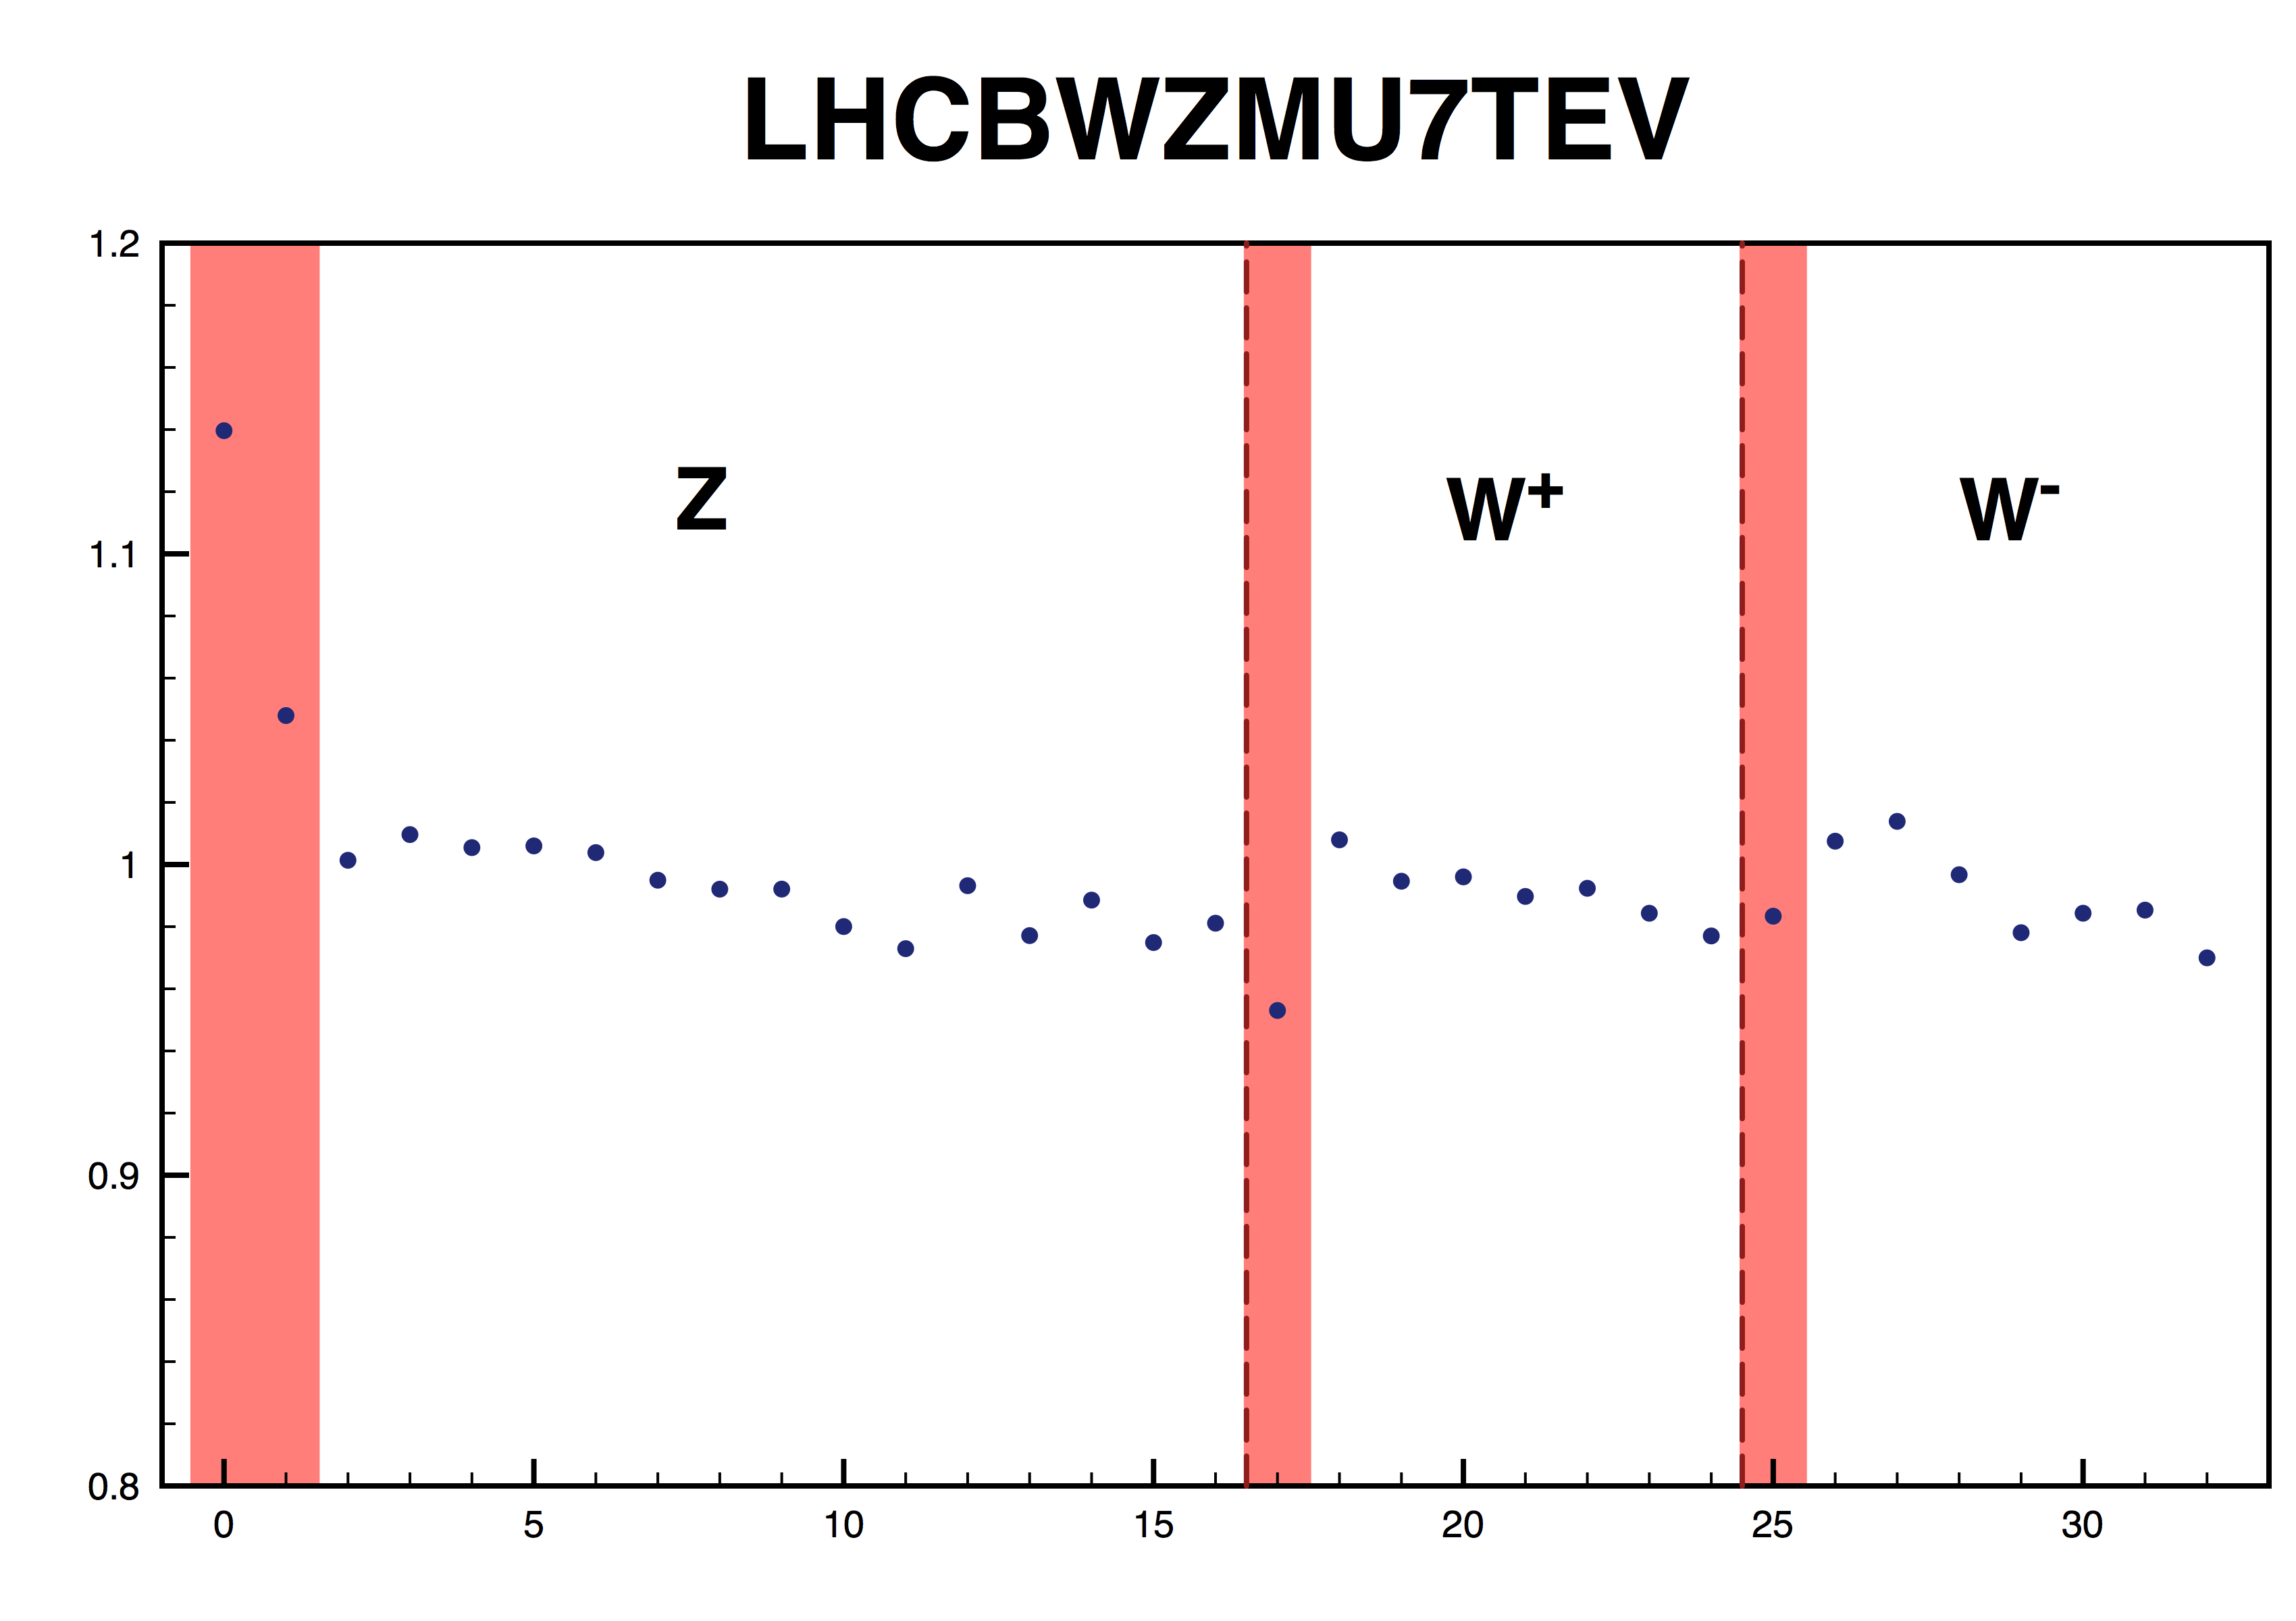
\includegraphics[width=0.49\linewidth]{images/plots/LHCBWZMU7TEV.png}
  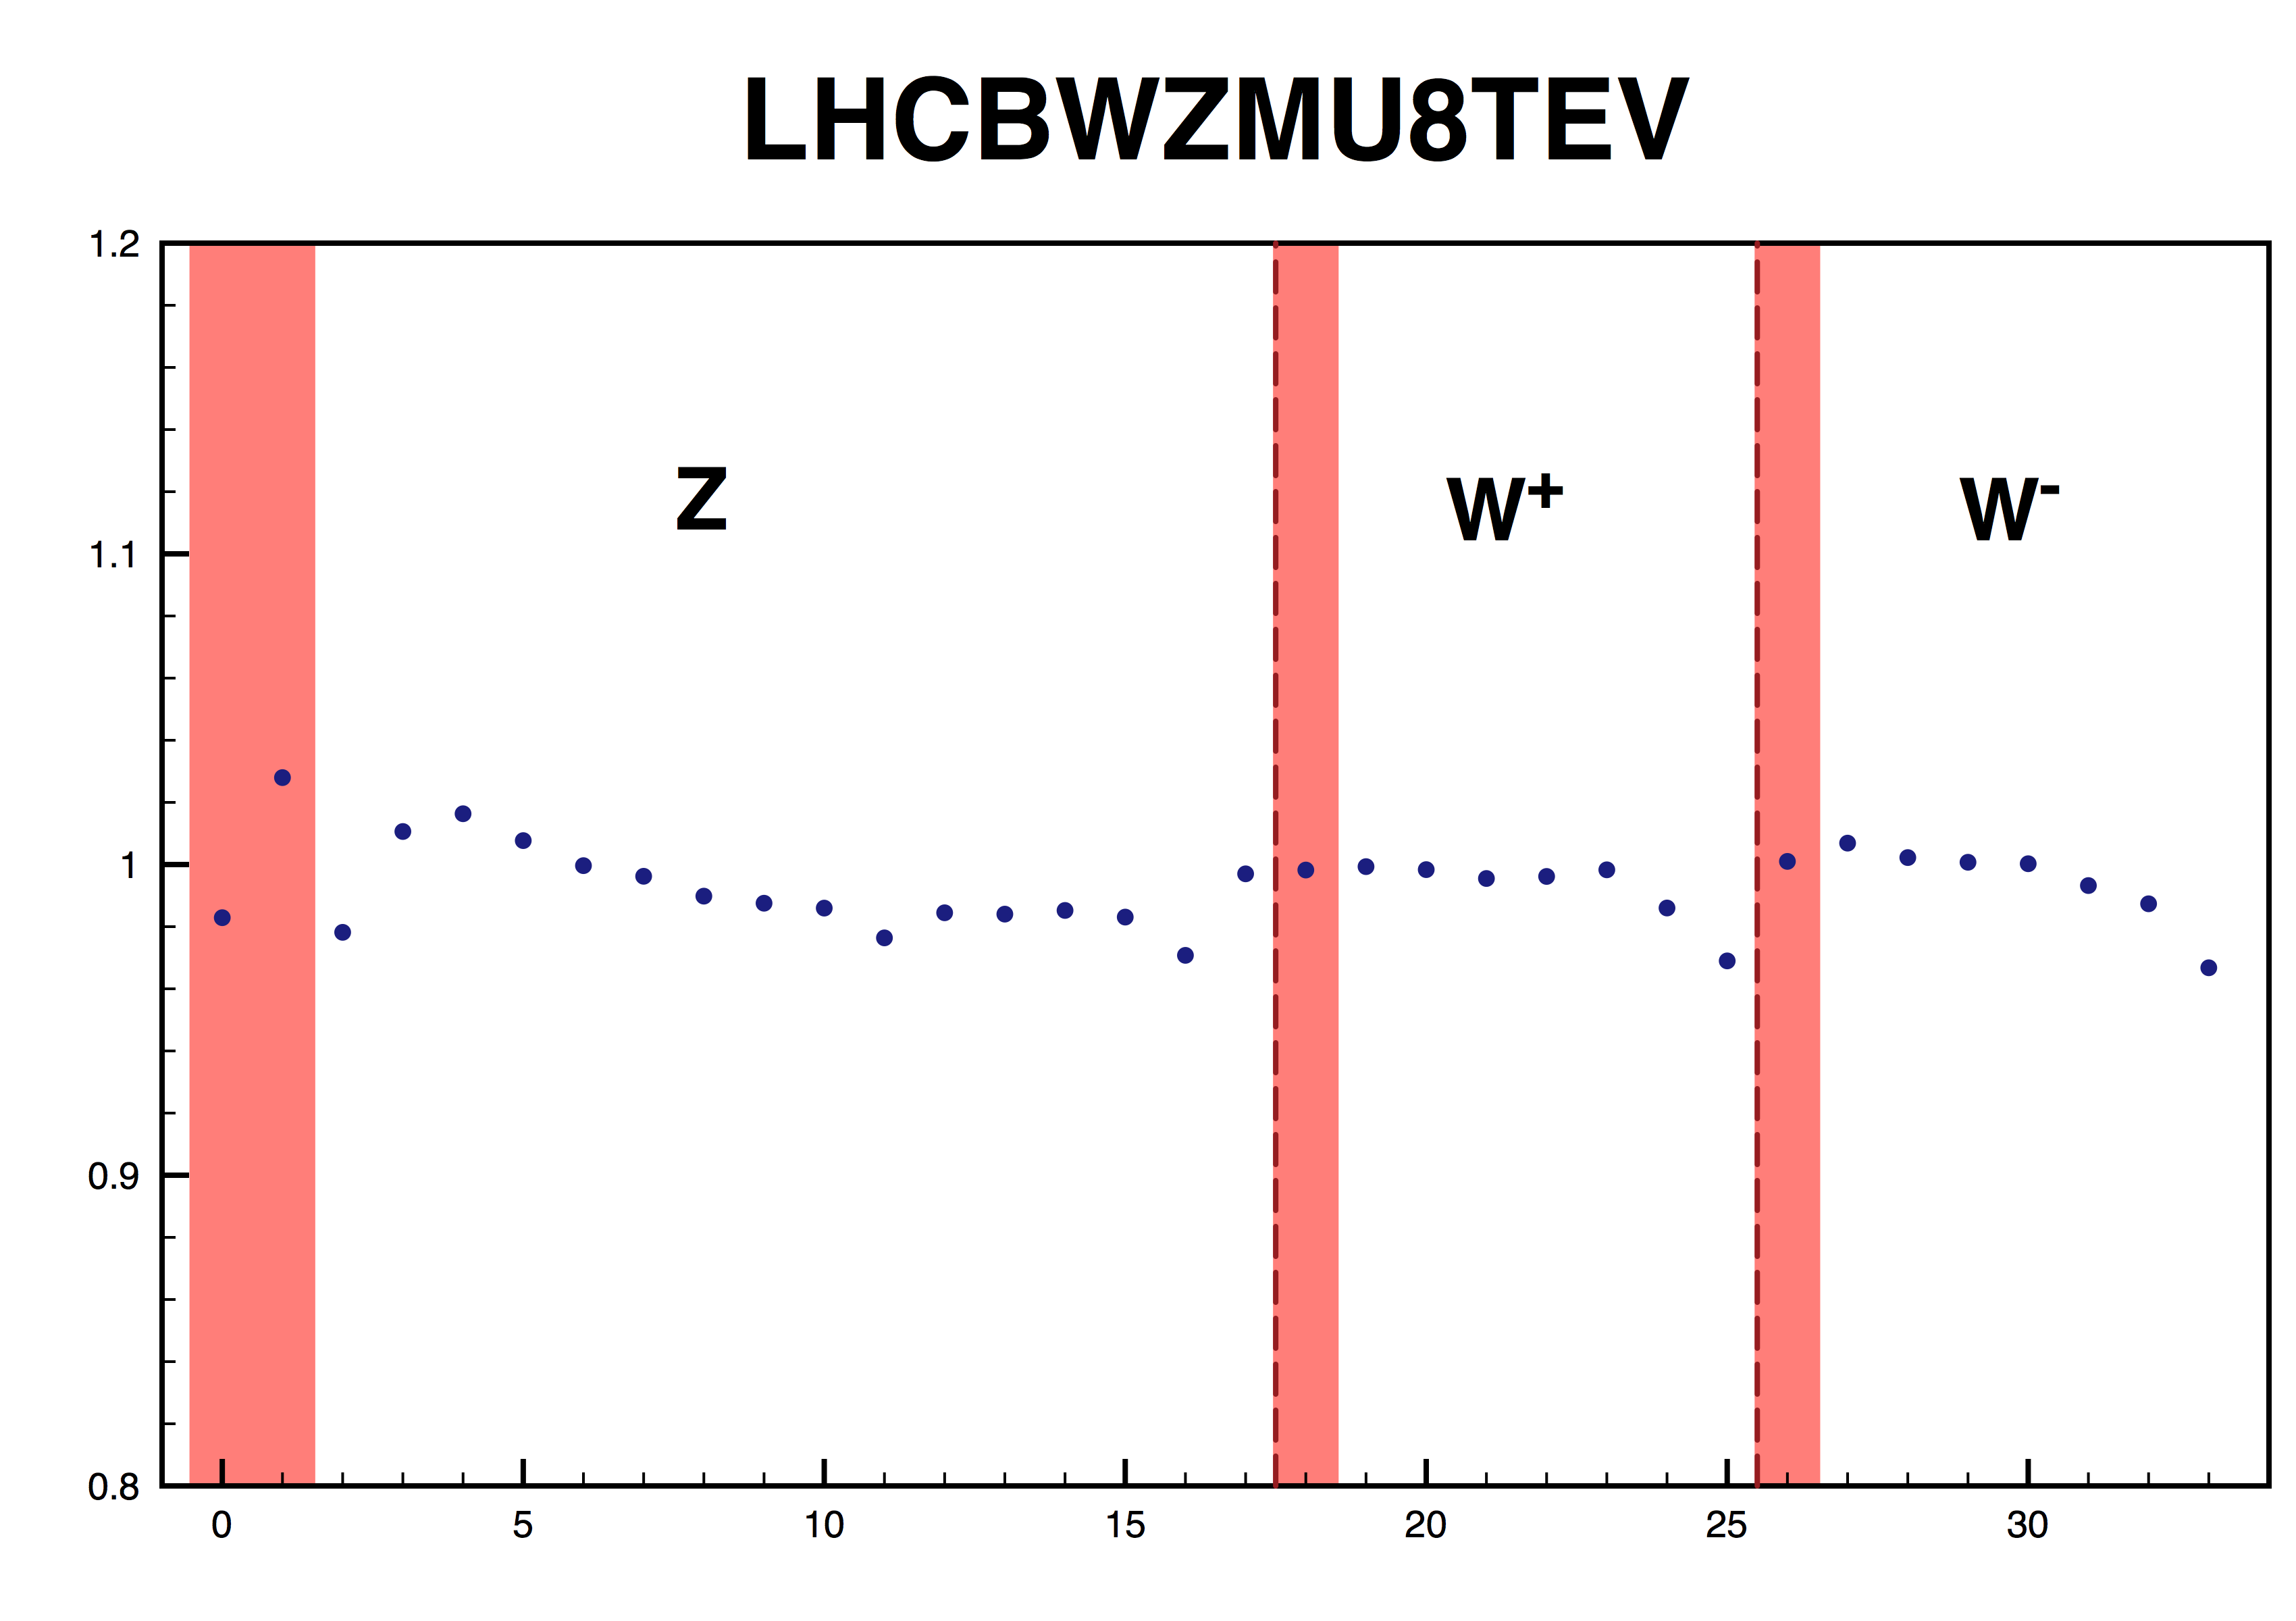
\includegraphics[width=0.49\linewidth]{images/plots/LHCBWZMU8TEV.png}
  \caption{\small   LHCb $7$（左）与 $8$~TeV（右）数据的 NNLO/NLO 截面比。被切割掉的中心快度区以红色阴影标出。
    \label{fig:lhcbcf}}
\end{center}
\end{figure}
%%%%%%%%%%%%%%%%%%%%%%%%%%%%%%%%%%%%%%%%%%%%%%%%%%%%%%%%%%%
LHCb 方面：NNPDF3.0 中的旧数据被 7~TeV 与 8~TeV $\mu$ 子道的最终版 $W+$、$W^-$ 与 $Z$ 快度分布~\cite{Aaij:2015gna,Aaij:2015zlq}取代。NNLO/NLO 截面比示于图~\ref{fig:lhcbcf}。
%
该数据集中 $|y_l|\le 2.25$ 的数据已被切割，因为异常偏大的 NNLO 修正提示它们可能不可靠。
理论预言在 NLO 用 MCFM 构造的 {\tt APPLgrids}得到，NNLO 修正用 {\tt FEWZ} 计算。



\subsection{$Z$ 玻色子的横向动量}
\label{sec:zpt}

得益于该过程最近的 NNLO 计算~\cite{Ridder:2015dxa,Ridder:2016nkl,Boughezal:2015ded,Boughezal:2016isb}，$Z$ 玻色子横向动量分布首次被纳入全局 PDF 确定。
在 NNPDF3.1 中，按照文献~\cite{Boughezal:2017nla}的细致研究，我们纳入了 ATLAS 与 CMS 的近期数据集。

%

ATLAS 已发表了 7~TeV~\cite{Aad:2014xaa}与 8~TeV~\cite{Aad:2015auj}的 $Z$
横向动量谱测量。测量在 $Z/\gamma^*\to e^+e^-$ 与 $Z/\gamma^*\to \mu^+\mu^-$ 两道进行后再行合并。7~TeV 数据基于 4.7~${\rm fb}^{-1}$ 积分亮度，8~TeV 数据基于 20.3~fb$^{-1}$。下面依次讨论这两个数据集。

7~TeV 数据取于 $Z$ 峰位处，$Z$ 横向动量最高达 $p_T^Z=800$ GeV。
%
数据以对直至 $|y_Z|=2.4$ 的 $Z/\gamma^*$ 快度单举给出，同时也在三个分离的快度 bin（$0.0\le |y_Z| \le 1.0$、$1.0 \le |y_Z| \le 2.0$、$2.0 \le |y_Z| \le 2.4$）给出。
%
为了最大化对 PDF 的潜在约束，只考虑微分测量。
%
测量以归一化截面 $(1/\sigma_Z)\,d\sigma(Z)/d p_T^Z$ 的形式给出，其中 $\sigma_Z$
是相应双轻子快度 bin 中的 fiducial 截面。
%
%该数据的特点是统计与系统不确定度相当小……（原文此处注释删）
该数据集因第~\ref{sec:impactzpt} 节将讨论的原因而未被纳入默认 NNPDF3.1 数据集。

8~TeV 数据集的 $p_T^Z$ 最高达 $900$~GeV，按三个不变质量 bin 给出：低于 $Z$ 峰的低质量区、峰上区，以及 $Z$ 峰以上直至 $\Mll=$ 150 GeV 的高质量区。
%
此外，峰位处的测量既有对整个快度范围 $0.0<|y_Z|<2.4$ 的单举形式，也有六个分离快度 bin（$0<y_Z<0.4$、$0.4<|y_Z|<0.8$、$0.8<|y_Z|<1.2$、$1.2<|y_Z|<1.6$、$1.6<|y_Z|<2.0$、$2.0<|y_Z|<2.4$）的微分形式。
%
此处再次采用更微分的测量。
%
与 7~TeV 数据不同，该数据集同时提供归一化与绝对两种分布。我们采用绝对分布，不仅因为它带有截面归一化的额外信息，也因为当用于计算归一化的数据所在范围与用于 PDF 确定的数据范围不一致时可能出现问题。该问题在文献~\cite{Boughezal:2017nla}中有详细讨论，并在第~\ref{sec:impactzpt} 节描述。

CMS 以 $\mu$ 子道、19.7 fb$^{-1}$ 积分亮度在 8~TeV~\cite{Khachatryan:2015oaa}测量了按 $p_T$ 与快度 $y_Z$ 微分的截面。
数据在五个快度 bin（$0.0<|y_Z|<0.4$、$0.4<|y_Z|<0.8$、$0.8<|y_Z|<1.2$、$1.2<|y_Z|<1.6$、$1.6<|y_Z|<2.0$）给出。
%
我们不考虑此前 CMS 在 7~TeV 的测量~\cite{Chatrchyan:2011wt}：它基于更小的数据集，且会与 NNPDF3.0 已纳入并被 NNPDF3.1 保留的双微分分布~\cite{Chatrchyan:2013tia}构成重复计数。


对数据施加三组运动学切割。
%
首先，保证固定阶微扰论的可靠性要求 $p_T^Z \ge$ 30 GeV（更小 $p_T$ 需要重求和）~\cite{Boughezal:2017nla}。
%
其次，剔除电弱修正很大且与实验数据可比的区域，要求 ATLAS~(CMS) 数据满足 $p_T^Z \le 150~(170)$ GeV~\cite{Boughezal:2017nla}。
%
最后，CMS 数据集中最大的快度 bin 因为与 ATLAS 同 bin 测量及理论预言都明显不相容而被舍弃。这种不相容的起源尚不清楚~\cite{Boughezal:2017nla}。

理论预言取自文献~\cite{Boughezal:2017nla}，其基于文献~\cite{Boughezal:2015ded,Boughezal:2016isb}的 $Z$+jet 产生 NNLO 计算。分解与重整化标度取为
\be
\mu_R=\mu_F =
\sqrt{(p_T)^2+\Mll^2} \, ,
\ee
其中 $\Mll$ 为末态轻子对不变质量。
%
该计算包括 $Z$ 与 $\gamma^*$ 贡献、它们的干涉及衰变到轻子对。对具有 ATLAS 与 CMS 接收度切割的观测量，NNLO/NLO 之比示于图~\ref{fig:zptcf}（用 NNPDF3.0 PDF、$\alpha_s(m_Z)=0.118$ 计算）：NNLO 修正从低 $p_T$ 的约 2--3\% 到高 $p_T$ 的约 10%，因此要以亚百分比精度描述数据必须计入该修正。
% 

%%%%%%%%%%%%%%%%%%%%%%%%%%%%%%%%%%%%%%%%%%%%%%%%%%%%%%%%%%%%%%%
\begin{figure}[t]
\begin{center}
  \includegraphics[width=0.49\linewidth]{images/plots/atlas7tev_CF.pdf}
  \includegraphics[width=0.49\linewidth]{images/plots/cms8tev_CF.pdf}\\
  \includegraphics[width=0.49\linewidth]{images/plots/atlas8tevy_CF.pdf}
  \includegraphics[width=0.49\linewidth]{images/plots/atlas8tevm_CF.pdf}
  \caption{\small   对应 ATLAS 7~TeV（左上）、CMS 8~TeV（右上）接收度切割与分 bin，以及 ATLAS 8 TeV 快度（左下）与不变质量（右下）分布的 $Z$ $p_T$ 数据 NNLO/NLO 截面比。
    \label{fig:zptcf}}
\end{center}
\end{figure}
%%%%%%%%%%%%%%%%%%%%%%%%%%%%%%%%%%%%%%%%%%%%%%%%%%%%%%%%%%%

即便是精度最高的 NNLO/NLO 修正因子仍然表现出涨落，如图~\ref{fig:zptcf}所示（图中画的是 8~TeV ATLAS 数据中心快度 bin 的 NNLO/NLO 截面比）。数据点连同其名义上的蒙特卡罗积分不确定度一起画出~\cite{Boughezal:2017nla}。
理论预言的点对点统计涨落似乎大于 ATLAS 数据典型的非关联统计不确定度——后者通常处于亚百分点甚至千分之一量级。为核查这一点，我们对截面比按固定快度下随 $p_T^Z$ 的变化拟合了一组神经网络。
对 ATLAS 与 CMS 数据的每个快度 bin 都进行了拟合；细节见文献~\cite{Carrazza:2017bjw}。
ATLAS 数据中心快度 bin 的拟合结果及其一倍标准差不确定度示于图~\ref{fig:cf-zpt-fit}。

 拟合的一倍标准差不确定度由 NNLO 计算的点对点涨落决定，达到百分之一量级，明显大于数据的统计不确定度。事实上，通过考察图~\ref{fig:zptcf}--\ref{fig:cf-zpt-fit} 可以清楚看到 NNLO/NLO 之比的点对点涨落远大于数据自身的涨落（如文献~\cite{Aad:2014xaa,Boughezal:2017nla}所见）。我们得出结论：NNLO 预言存在残余理论不确定度，我们估计对所有数据集约为 1\%。该结论已通过改变切割或函数形式重复拟合得到验证与交叉核对。因此我们给该数据集额外添加了 1\% 的完全不关联理论不确定度（另见文献~\cite{Boughezal:2017nla}）。

%%%%%%%%%%%%%%%%%%%%%%%%%%%%%%%%%%%%%%%%%%%%%%%%%%%%%%%%%%%%%%%
\begin{figure}[t]
\begin{center}
  \includegraphics[scale=0.55]{images/plots/cf-zpt-fit.pdf}
  \caption{\small
    8~TeV ATLAS $Z$ $p_T$ 分布中心快度 bin 的 NNLO/NLO 截面比。图中还给出拟合结果及其相应不确定度。
\label{fig:cf-zpt-fit}}
\end{center}
\end{figure}
%%%%%%%%%%%%%%%%%%%%%%%%%%%%%%%%%%%%%%%%%%%%%%%%%%%%%%%%%%%

\subsection{$t\bar{t}$ 产生的微分分布与总截面}
\label{sec:topdata}

依照文献~\cite{Czakon:2016olj}的细致研究，顶夸克对产生的微分分布已被纳入 NNPDF3.1。
ATLAS 与 CMS 用多种运动学变量测量了这些分布，包括顶夸克快度 $y_t$、顶夸克对快度 $y_{t\bar{t}}$、顶夸克横向动量 $p_T^t$ 以及 top-antitop 系统不变质量 $m_{t\bar{t}}$。ATLAS 同时提供绝对与归一化微分分布，而 CMS 只提供归一化结果。
%
所有这些分布的微扰 QCD 修正在 NNLO 已被算出~\cite{Czakon:2015owf,Czakon:2016dgf}。
%
为避免重复计数，每个实验只能有一种分布进入数据集，因为不同分布之间的统计关联未知。
%
NNPDF3.1 采用的微分分布选择遵循文献~\cite{Czakon:2016olj}的建议，那里系统研究了各种顶夸克对微分分布组合对胶子 PDF 的影响。
%
研究发现归一化快度分布约束力最强，并且使 ATLAS 与 CMS 的理论与数据符合良好。
%
使用快度分布还有一些别的优点。
%
第一，降低可能的 BSM 效应污染的风险。
%
例如，重共振态会在快度分布中被运动学压低，但在 $m_{t\bar{t}}$ 与 $p_T^t$ 分布的尾部则不然。
%
第二，与 $p_T^t$ 及 $m_{t\bar{t}}$ 分布相比，快度分布对 $m_t$ 变化的敏感性较温和~\cite{Czakon:2016vfr}。

因此我们纳入 ATLAS~\cite{Aad:2015mbv}与 CMS~\cite{Khachatryan:2015oqa}的 8~TeV 轻子+喷注末态归一化快度分布，分别对应 20.3 fb$^{-1}$ 与 19.7 fb$^{-1}$ 的积分亮度。
%
我们考虑全相空间测量，观测量用顶夸克或顶夸克对运动学变量重构，因为 NNLO 结果只对稳定顶夸克可用。
我们还依照文献~\cite{Czakon:2016olj}纳入 ATLAS~\cite{Aad:2014kva,Aaboud:2016pbd}与 CMS~\cite{Khachatryan:2016mqs,CMS:2016syx}在 $7$、$8$、$13$~TeV 的最新总截面测量。
%
它们取代了 NNPDF3.0 中纳入的
ATLAS~\cite{ATLAS:2012aa,ATLAS:2011xha,TheATLAScollaboration:2013dja}与
CMS~\cite{Chatrchyan:2013faa,Chatrchyan:2012bra,Chatrchyan:2012ria}先前测量。

NLO 理论预言用 {\tt Sherpa}~\cite{Gleisberg:2008ta}生成，格式与 {\tt APPLgrid}~\cite{Carli:2010rw}兼容，使用 {\tt MCgrid}~\cite{DelDebbio:2013kxa}代码与 {\tt Rivet}~\cite{Buckley:2010ar}分析包，NLO 矩阵元来自 {\tt OpenLoops}~\cite{Cascioli:2011va}。
%
所有计算都采用很大的蒙特卡罗积分样本量，以保证残余数值涨落可忽略。
%
我们的结果已与文献~\cite{Czakon:2016dgf}程序的输出仔细基准比对。
%
重整化与分解标度 $\mu_R$、$\mu_F$ 按文献~\cite{Czakon:2016dgf}的建议取为
\be
\label{eq:scale1}
\mu_R=\mu_F=\mu=H_T/4 \, , \qquad H_T \equiv \sqrt{m_t^2+\lp {p_T^t}\rp^2}
+ \sqrt{m_t^2+\lp {p_T^{\bar{t}}}\rp^2} \, ,
\ee
其中 $m_t=173.3$ GeV 为顶夸克极点质量的 PDG 世界平均值~\cite{Agashe:2014kda}，$p_T^t$（$p_T^{\bar{t}}$）为顶（反顶）横向动量。
归一化微分分布的 NLO 理论预言由绝对分布除以在数据运动学范围内积分的截面得到。


NNLO 修正因子对绝对微分截面及其归一化总截面分别计算。
%
微分截面用文献~\cite{Czakon:2016dgf}的程序并以式~(\ref{eq:scale1})的标度选择确定。
%
NNLO/NLO 之比的结果示于图~\ref{fig:ttbar-cfact}：可见 NNLO 修正大小为 6\% 与 9\%，实际上小于数据不确定度，并且在数据覆盖的运动学区域内形状相当平坦。
我们还通过使用三个不同全局 PDF 集合明确展示了结果对计算所用 PDF 集合的依赖：可见该依赖完全可忽略。

总截面用 {\tt top++}~\cite{Czakon:2011xx}以 NNLO+NNLL 计算，固定标度 $\mu_R=\mu_F=m_t$，遵循文献~\cite{Czakon:2016dgf}的建议，即当 NNLO 微分分布用动力学标度确定时，应搭配 NNLO+NNLL 重求和截面使用。



%

%%%%%%%%%%%%%%%%%%%%%%%%%%%%%%%%%%%%%%%%%%%%%%%%%%%%%%%%%%%%%%%
\begin{figure}[t]
\begin{center}
  \includegraphics[scale=0.31,angle=270]{images/plots/ttbar-cfact_yt.pdf}
  \includegraphics[scale=0.31,angle=270]{images/plots/ttbar-cfact_ytt.pdf}\\
  \caption{\small
    对应 8~TeV ATLAS 与 CMS 数据的顶夸克快度 $y_t$（左）
    与顶夸克对快度 $y_{t\bar{t}}$（右）的 NNLO/NLO 截面比。
    %
     图中给出用三种输入 PDF 集合（NNPDF3.0、CT14 与 MMHT14）所得的结果。
\label{fig:ttbar-cfact}}
\end{center}
\end{figure}
%%%%%%%%%%%%%%%%%%%%%%%%%%%%%%%%%%%%%%%%%%%%%%%%%%%%%%%%%%%




